% move all configuration stuff into includes file so we can focus on the content
\documentclass[aspectratio=169,hyperref={pdfpagelabels=false,colorlinks=true,linkcolor=white,urlcolor=blue},t]{beamer}

%%%%%%%%%%%%%%%%%%%%%%%%%%%%%%%%%%%%%%%%%%%%%%%%%%%%%%%%%%%%%%%%%%%%%%%%%%%%%%%%%%
%%%%%%%%%%%%%%%%%%%%%%%%%%%%%%%%%%%%%%%%%%%%%%%%%%%%%%%%%%%%%%%%%%%%%%%%%%%%%%%%%%
% packages
\usepackage{pict2e}
\usepackage{epic}
\usepackage{amsmath,amsfonts,amssymb}
\usepackage{units}
\usepackage{fancybox}
\usepackage[absolute,overlay]{textpos} 
\usepackage{media9} % avi2flv: "C:\Program Files\ffmpeg\bin\ffmpeg.exe" -i TuneFreqFilterbank.avi -b 600k -s 441x324 -r 15 -acodec copy TuneFreqFilterbank.flv
\usepackage{animate}
\usepackage{gensymb}
\usepackage{multirow}
\usepackage{silence}
\usepackage[backend=bibtex,style=ieee]{biblatex}
\AtEveryCitekey{\iffootnote{\tiny}{}}
\addbibresource{references}

%%%%%%%%%%%%%%%%%%%%%%%%%%%%%%%%%%%%%%%%%%%%%%%%%%%%%%%%%%%%%%%%%%%%%%%%%%%%%%%%%%
%%%%%%%%%%%%%%%%%%%%%%%%%%%%%%%%%%%%%%%%%%%%%%%%%%%%%%%%%%%%%%%%%%%%%%%%%%%%%%%%%%
% relative paths
\graphicspath{{graph/}}


%%%%%%%%%%%%%%%%%%%%%%%%%%%%%%%%%%%%%%%%%%%%%%%%%%%%%%%%%%%%%%%%%%%%%%%%%%%%%%%%%%
%%%%%%%%%%%%%%%%%%%%%%%%%%%%%%%%%%%%%%%%%%%%%%%%%%%%%%%%%%%%%%%%%%%%%%%%%%%%%%%%%%
% units
\setlength{\unitlength}{1mm}

%%%%%%%%%%%%%%%%%%%%%%%%%%%%%%%%%%%%%%%%%%%%%%%%%%%%%%%%%%%%%%%%%%%%%%%%%%%%%%%%%%
%%%%%%%%%%%%%%%%%%%%%%%%%%%%%%%%%%%%%%%%%%%%%%%%%%%%%%%%%%%%%%%%%%%%%%%%%%%%%%%%%%
% theme & layout
\usetheme{Frankfurt}
\beamertemplatenavigationsymbolsempty
%\setbeamertemplate{frametitle}[smoothbars theme]
\setbeamertemplate{frametitle}
{
    \begin{beamercolorbox}[ht=1.8em,wd=\paperwidth]{frametitle}
        \vspace{-.1em}%
        \hspace{.2em}{\strut\insertframetitle\strut}
        
        \hspace{.2em}\small\strut\insertframesubtitle\strut
        %\hfill
        %
\includegraphics[height=.8cm,keepaspectratio]{CenterMusicTechnology-solid-2lines-white-CoAtag}
        
    \end{beamercolorbox}
    \begin{textblock*}{100mm}(11.6cm,.7cm)
        \includegraphics[height=.8cm,keepaspectratio]{logo_GTCMT_black}
    \end{textblock*}
}

% set this to ensure bulletpoints without subsections
\usepackage{remreset}
\makeatletter
\@removefromreset{subsection}{section}
\makeatother
\setcounter{subsection}{1}

%---------------------------------------------------------------------------------
% appearance
\setbeamercolor{structure}{fg=gtgold}
\setbeamercovered{transparent} %invisible
\setbeamercolor{bibliography entry author}{fg=black}
\setbeamercolor*{bibliography entry title}{fg=black}
\setbeamercolor*{bibliography entry note}{fg=black}

%\usepackage{pgfpages}
%\setbeameroption{show notes}
%\setbeameroption{show notes on second screen=right}
%---------------------------------------------------------------------------------
% fontsize
\let\Tiny=\tiny

%%%%%%%%%%%%%%%%%%%%%%%%%%%%%%%%%%%%%%%%%%%%%%%%%%%%%%%%%%%%%%%%%%%%%%%%%%%%%%%%%%
%%%%%%%%%%%%%%%%%%%%%%%%%%%%%%%%%%%%%%%%%%%%%%%%%%%%%%%%%%%%%%%%%%%%%%%%%%%%%%%%%%
% warnings
\pdfsuppresswarningpagegroup=1
\WarningFilter{biblatex}{Patching footnotes failed}
\WarningFilter{latexfont}{Font shape}
\WarningFilter{latexfont}{Some font shapes}
\WarningFilter{gensymb}{Not defining}


%%%%%%%%%%%%%%%%%%%%%%%%%%%%%%%%%%%%%%%%%%%%%%%%%%%%%%%%%%%%%%%%%%%%%%%%%%%%%%%%%%
%%%%%%%%%%%%%%%%%%%%%%%%%%%%%%%%%%%%%%%%%%%%%%%%%%%%%%%%%%%%%%%%%%%%%%%%%%%%%%%%%%
% title information
\title[]{Introduction to Audio Content Analysis}   
\author[alexander lerch]{alexander lerch} 
%\institute{~}
%\date[Alexander Lerch]{}
\titlegraphic{\vspace{-16mm}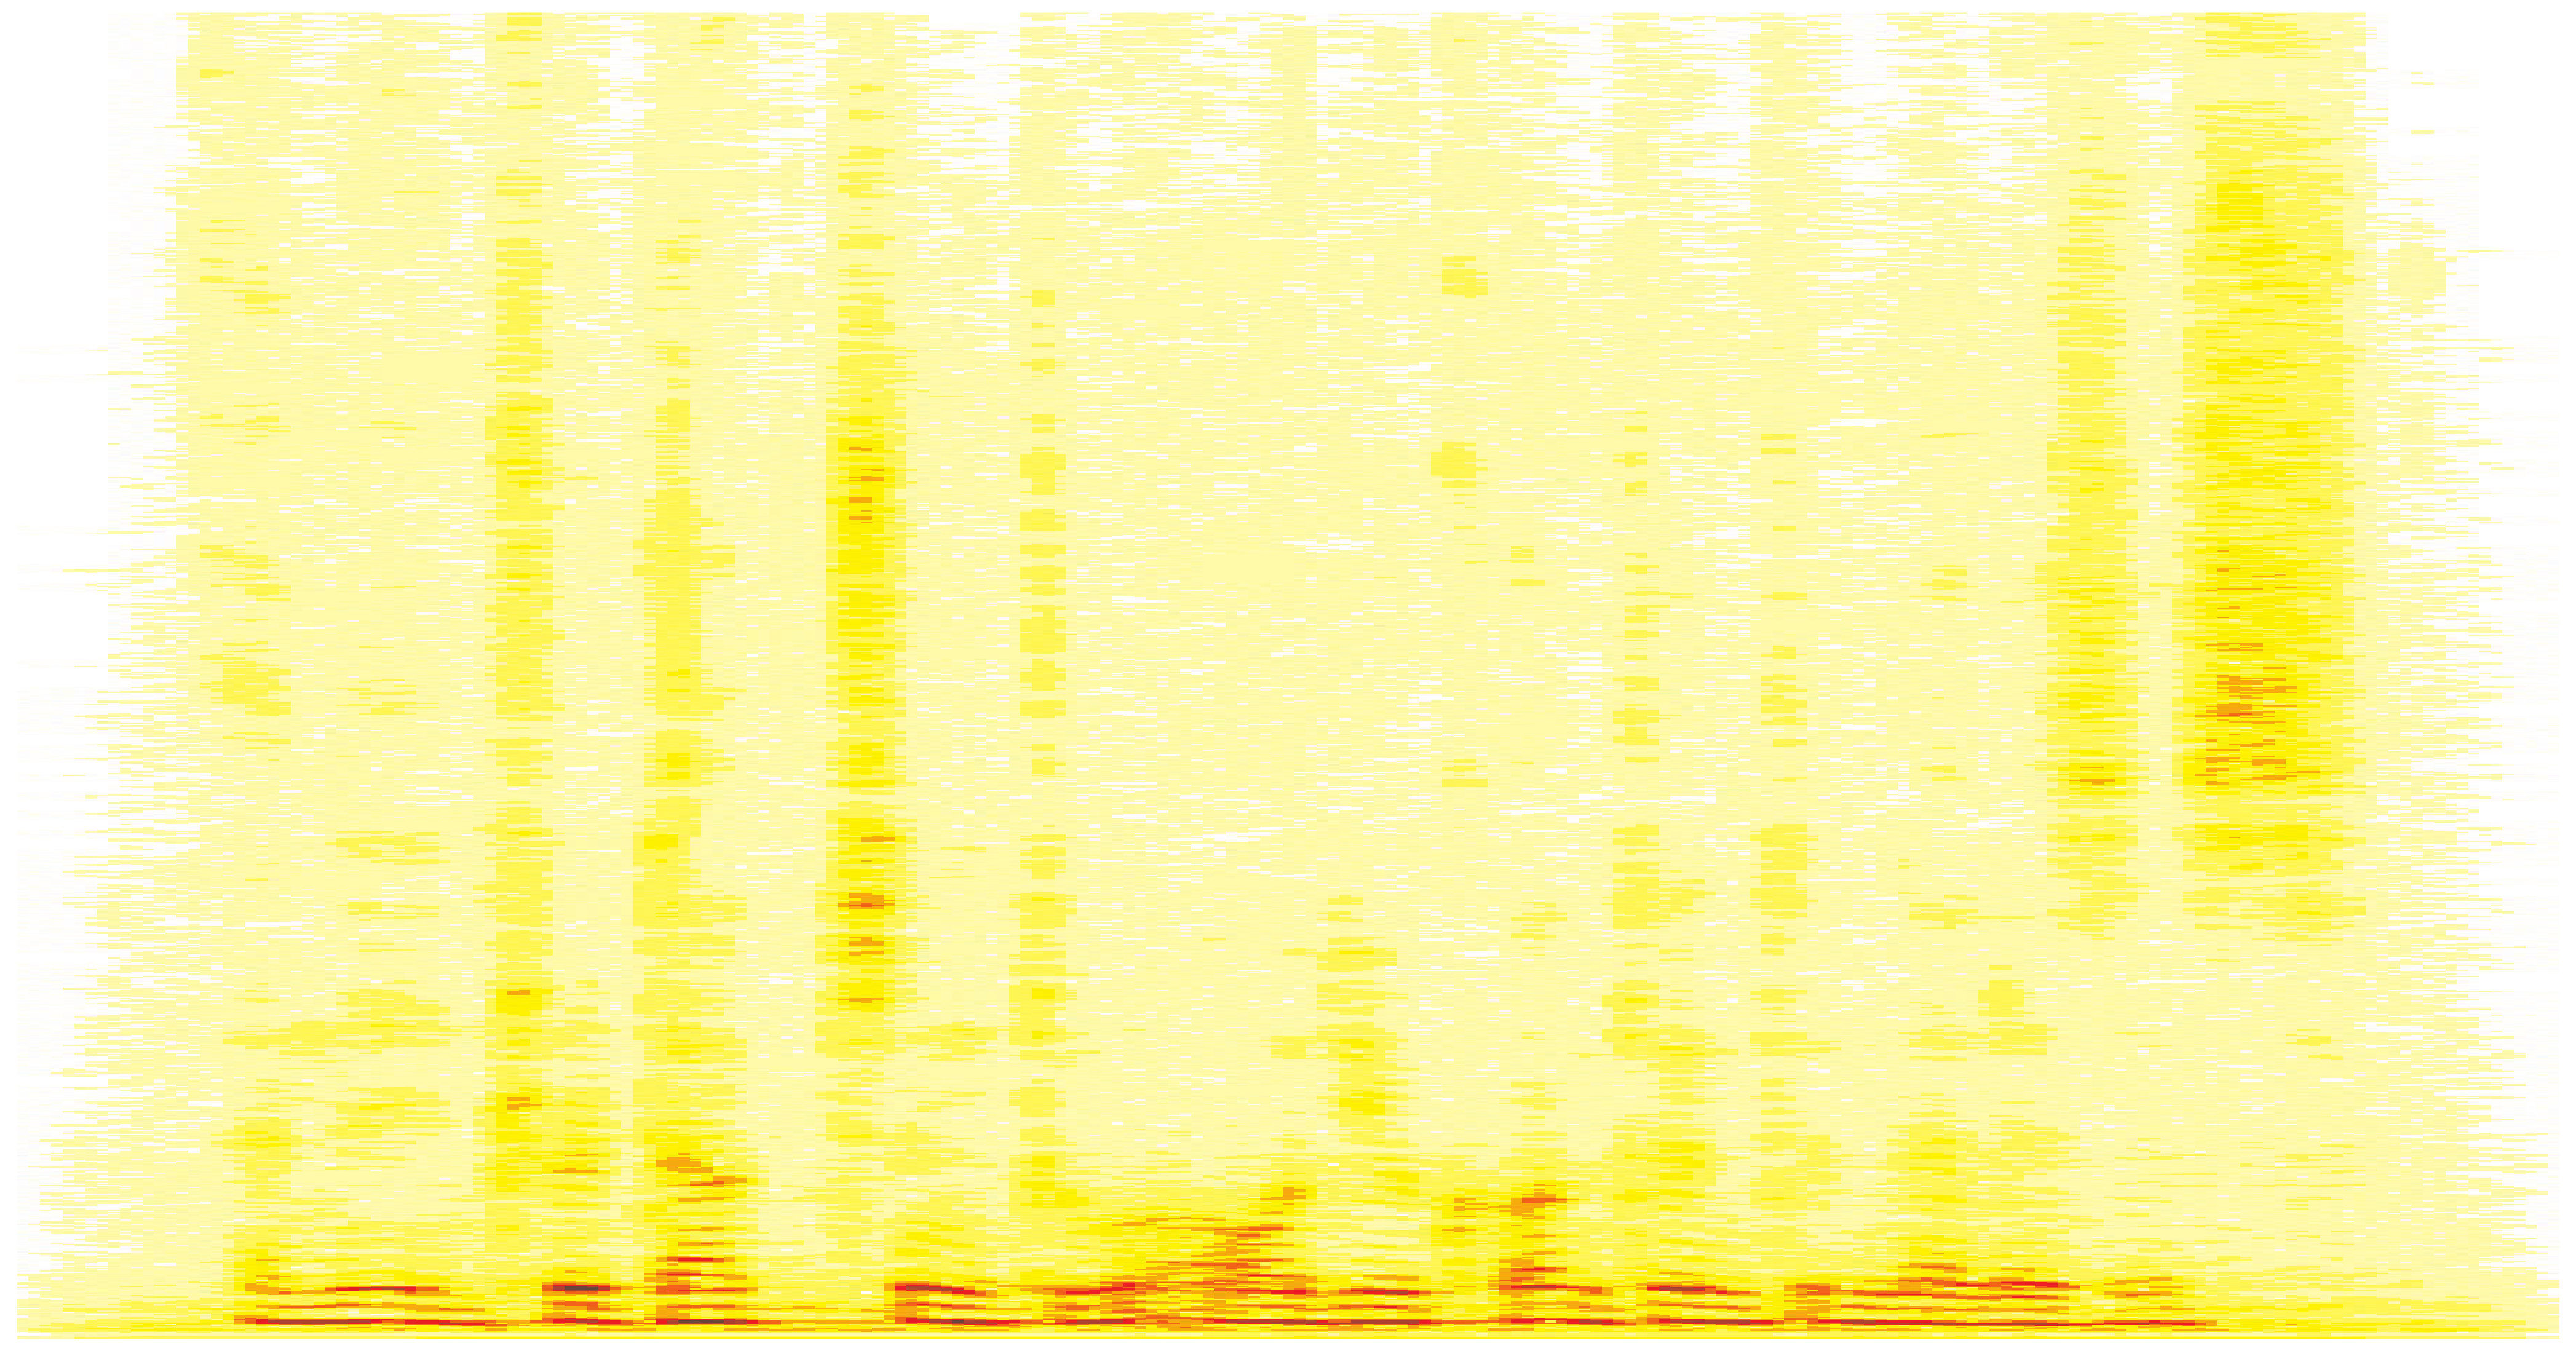
\includegraphics[width=\textwidth,height=3cm]{title}}

%%%%%%%%%%%%%%%%%%%%%%%%%%%%%%%%%%%%%%%%%%%%%%%%%%%%%%%%%%%%%%%%%%%%%%%%%%%%%%%%%%
%%%%%%%%%%%%%%%%%%%%%%%%%%%%%%%%%%%%%%%%%%%%%%%%%%%%%%%%%%%%%%%%%%%%%%%%%%%%%%%%%%
% colors
\definecolor{gtgold}{HTML}{E0AA0F} %{rgb}{0.88,0.66,1,0.06} [234, 170, 0]/256

%%%%%%%%%%%%%%%%%%%%%%%%%%%%%%%%%%%%%%%%%%%%%%%%%%%%%%%%%%%%%%%%%%%%%%%%%%%%%%%%%%
%%%%%%%%%%%%%%%%%%%%%%%%%%%%%%%%%%%%%%%%%%%%%%%%%%%%%%%%%%%%%%%%%%%%%%%%%%%%%%%%%%
% math
\DeclareMathOperator*{\argmax}{argmax}
\DeclareMathOperator*{\argmin}{argmin}
\DeclareMathOperator*{\atan}{atan}
\DeclareMathOperator*{\arcsinh}{arcsinh}
\DeclareMathOperator*{\sign}{sign}
\DeclareMathOperator*{\tcdf}{tcdf}
\DeclareMathOperator*{\si}{sinc}
\DeclareMathOperator*{\princarg}{princarg}
\DeclareMathOperator*{\arccosh}{arccosh}
\DeclareMathOperator*{\hwr}{HWR}
\DeclareMathOperator*{\flip}{flip}
\DeclareMathOperator*{\sinc}{sinc}
\DeclareMathOperator*{\floor}{floor}
\newcommand{\e}{{e}}
\newcommand{\jom}{\mathrm{j}\omega}
\newcommand{\jOm}{\mathrm{j}\Omega}
\newcommand   {\mat}[1]    		{\boldsymbol{\uppercase{#1}}}		%bold
\renewcommand {\vec}[1]    		{\boldsymbol{\lowercase{#1}}}		%bold

%%%%%%%%%%%%%%%%%%%%%%%%%%%%%%%%%%%%%%%%%%%%%%%%%%%%%%%%%%%%%%%%%%%%%%%%%%%%%%%%%%
%%%%%%%%%%%%%%%%%%%%%%%%%%%%%%%%%%%%%%%%%%%%%%%%%%%%%%%%%%%%%%%%%%%%%%%%%%%%%%%%%%
% media9
\newcommand{\includeaudio}[1]{{\includemedia[
                        addresource=audio/#1.mp3,
                        width=5mm,
                        height=5mm,
                        activate=onclick,
                        flashvars={
                            source=audio/#1.mp3  
                            &autoPlay=true
                        }]
                        {
\includegraphics[width=5mm, height=5mm]{SpeakerIcon}}
                        {APlayer.swf}}}
\newcommand{\audioautoplay}[1]{{\begin{center}\includemedia[
                            addresource=audio/#1.mp3,
                            width=.1\linewidth,
                            height=.01\linewidth,
                            activate=pageopen,
                            flashvars={
                                source=audio/#1.mp3  
                                &autoPlay=true
                            }]
                            {}
                            {APlayer.swf}\end{center}}}

\newcommand{\includevideo}[1]{{\begin{center}\includemedia[
                        addresource=video/#1.mp4,
                        width=0.8\linewidth,
                        height=0.4\linewidth,
                        activate=onclick,
                        flashvars={
                            source=video/#1.mp4  
                            &autoPlay=true
                        }]
                        {}
                        {VPlayer.swf}\end{center}}}
\newcommand{\videowithmatlab}[1]{{\begin{center}\includemedia[
                        addresource=video/animate#1.mp4,
                        width=0.8\linewidth,
                        height=0.4\linewidth,
                        activate=onclick,
                        flashvars={
                            source=video/animate#1.mp4  
                            &autoPlay=true
                        }]
                        {}
                        {VPlayer.swf}\end{center}\addreference{matlab source: matlab/animate#1.m}}}
                        

%%%%%%%%%%%%%%%%%%%%%%%%%%%%%%%%%%%%%%%%%%%%%%%%%%%%%%%%%%%%%%%%%%%%%%%%%%%%%%%%%%
%%%%%%%%%%%%%%%%%%%%%%%%%%%%%%%%%%%%%%%%%%%%%%%%%%%%%%%%%%%%%%%%%%%%%%%%%%%%%%%%%%
% other commands
\newcommand{\question}[1]{%\vspace{-4mm}
                          \setbeamercovered{invisible}
                          \begin{columns}[T]
                            \column{.8\textwidth}
                                \textbf{#1}
                            \column{.2\textwidth}
                                \vspace{-8mm}
                                \begin{flushright}
                                     
\includegraphics[scale=.5]{question_mark}
                                \end{flushright}
                                \vspace{6mm}
                          \end{columns}\pause\vspace{-12mm}}

\newcommand{\toremember}[1]{%\vspace{-4mm}
                          \begin{columns}[T]
                            \column{.8\textwidth}
                                \textbf{#1}
                            \column{.2\textwidth}
                                \vspace{-4mm}
                                \begin{flushright}
                                     
\includegraphics[scale=.5]{exclamation_mark}
                                \end{flushright}
                                \vspace{6mm}
                          \end{columns}\vspace{-6mm}}

\newcommand{\matlabexercise}[1]{%\vspace{-4mm}
                          \setbeamercovered{invisible}
                          \begin{columns}[T]
                            \column{.8\textwidth}
                                \textbf{matlab exercise}: #1
                            \column{.2\textwidth}
                                \begin{flushright}
                                     
\includegraphics[scale=.5]{logo_matlab}
                                \end{flushright}
                                %\vspace{6mm}
                          \end{columns}}

\newcommand{\addreference}[1]{  
                  
                    \begin{textblock*}{\baselineskip }(1.12\textwidth,.3\textheight) %(1.15\textwidth,.4\textheight)
                        \rotatebox{90}{\tiny {#1}}
                    \end{textblock*}}
                    
\newcommand{\figwithmatlab}[1]{
                    \begin{figure}
                        \centering
                        \includegraphics{#1}
                        %\label{fig:#1}
                    \end{figure}
                    
                    \addreference{matlab source: \href{https://github.com/alexanderlerch/ACA-Slides/blob/master/matlab/display#1.m}{matlab/display#1.m}}}
\newcommand{\figwithref}[2]{
                    \begin{figure}
                        \centering
                        \includegraphics{#1}
                        \label{fig:#1}
                    \end{figure}
                    
                    \addreference{#2}}  
                                    
\newcommand{\inserticon}[1]{

                    \begin{textblock*}{100mm}(14.5cm,7.5cm)
                        \includegraphics[height=.8cm,keepaspectratio]{#1}
                    \end{textblock*}}            

%%%%%%%%%%%%%%%%%%%%%%%%%%%%%%%%%%%%%%%%%%%%%%%%%%%%%%%%%%%%%%%%%%%%%%%%%%%%%%%%%%
%%%%%%%%%%%%%%%%%%%%%%%%%%%%%%%%%%%%%%%%%%%%%%%%%%%%%%%%%%%%%%%%%%%%%%%%%%%%%%%%%%
% counters
\newcounter{i}
\newcounter{j}
\newcounter{iXOffset}
\newcounter{iYOffset}
\newcounter{iXBlockSize}
\newcounter{iYBlockSize}
\newcounter{iYBlockSizeDiv2}
\newcounter{iDistance}



\subtitle{Module 2.0: Fundamentals~---~Signals}

%%%%%%%%%%%%%%%%%%%%%%%%%%%%%%%%%%%%%%%%%%%%%%%%%%%%%%%%%%%%%%%%%%%%%%%%%%%%
\begin{document}
    % generate title page
	

\begin{frame}
    \titlepage
    %\vspace{-5mm}
    \begin{flushright}
        \href{http://www.gtcmt.gatech.edu}{\includegraphics[height=.8cm,keepaspectratio]{logo_GTCMT_black}}
    \end{flushright}
\end{frame}


    \section[overview]{lecture overview}
        \begin{frame}{introduction}{overview}
            \begin{block}{corresponding textbook section}
                    \href{http://ieeexplore.ieee.org/xpl/articleDetails.jsp?tp=&arnumber=6331119&}{Chapter 2~---~Fundamentals}: pp.~7--9
                    \href{http://ieeexplore.ieee.org/xpl/articleDetails.jsp?tp=&arnumber=6331119&}{Chapter 2~---~Fundamentals}: pp.~13--14
            \end{block}

            \begin{itemize}
                \item   \textbf{lecture content}
                    \begin{itemize}
                        \item   deterministic \& periodic signals
                        \item   Fourier Series
                        \item   random signals
                    \end{itemize}
                \bigskip
                \item<2->   \textbf{learning objectives}
                    \begin{itemize}
                        \item   knowledge of basic signal categories
                        \item   understanding of every periodic signal comprising fundamental frequency and harmonics at integer multiples
                        \item   basic interpretation of the Fourier Series
                    \end{itemize}
            \end{itemize}
            \inserticon{directions}
        \end{frame}
        
    \section[intro]{introduction}
        \begin{frame}{audio signals}{signal categories}
            \begin{itemize}
                \item	\textbf{deterministic signals}:\\
                        \textit{predictable}: future shape of the signal can be known (example: sinusoidal)
                \pause		
                \item	\textbf{random signals}:\\
                        \textit{unpredictable}: no knowledge can help to predict what is coming next (example: white noise)
            \end{itemize}
            
            \bigskip
            \pause
            ``real-world'' audio signals can be modeled as time-variant combination of 
            \begin{itemize}
                \item	(quasi-)periodic parts
                \item	(quasi-)random parts
            \end{itemize}
        \end{frame}

    \section[periodic signals]{periodic signals}
        \begin{frame}{audio signals}{periodic signals 1/5}
            \setbeamercovered{invisible}
            \vspace{-2mm}
            periodic signals: most prominent examples of deterministic signals
            \begin{eqnarray*}
                x(t) 	&=& x(t+T_0)\\
                f_0 	&=& \frac{1}{T_0} =  \frac{\omega_0}{2\pi}
            \end{eqnarray*}

            \vspace{-4mm}
            \only<2>{
                \figwithmatlab{PeriodicRandom}
             }
            \vphantom{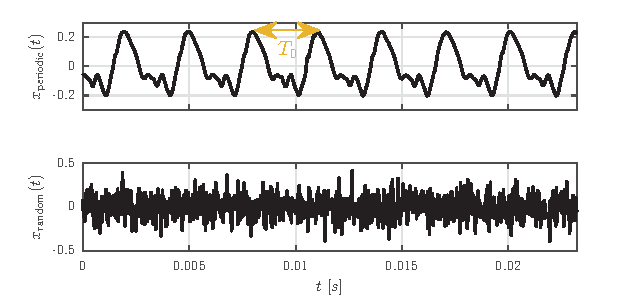
\includegraphics{PeriodicRandom}}
        \end{frame}

        \begin{frame}{audio signals}{periodic signals 2/5}
            periodic signal $\Rightarrow$ representation in \textbf{Fourier series}\footnote{\tiny Jean-Baptiste Joseph Fourier, 1768--1830}
            \begin {equation*}
                x(t) = \sum\limits_{k=-\infty}^{\infty} {\color<5>{gtgold}{a_k}} {\color<4>{gtgold}{\e^{\mathrm{j}{\color<2-3>{gtgold}{\omega_0}} {\color<3>{gtgold}{k}} t}}} \nonumber
            \end {equation*}
            \begin{itemize}
                \item<2-> $\omega_0 = 2\pi\cdot f_0$
                \item<3-> $k\omega_0$: integer multiples of the lowest frequency
                \item<4-> $\e^{\jom_0kt} = \cos(\omega_0kt) + \mathrm{j} \sin(\omega_0kt)$
                \item<5-> $a_k$: Fourier coefficients --- amplitude of each component
                    \begin {equation*}\label{eq:fourier_coeff}
                        a_k = \frac{1}{T_0}\int\limits_{-\nicefrac{T_0}{2}}^{\nicefrac{T_0}{2}} x(t) \e^{-\jom_0kt}\, dt \nonumber
                    \end {equation*}
            \end{itemize}
        \end{frame}

        \begin{frame}{audio signals}{periodic signals 3/5}
            \begin{block}{Fourier series}
                \begin{itemize}
                    \item   \textbf{every} periodic signal can be represented in a Fourier series
                    \item   a periodic signal \textbf{contains only} frequencies at integer multiples of the fundamental frequency $f_0$
                    \bigskip
                    \item<2->   Fourier series can only be applied to periodic signals
                    \item<2->   Fourier series is analytically elegant but only of limited practical use as the fundamental period has to be known
                \end{itemize}
            \end{block}
            \inserticon{lightbulb}
        \end{frame}

        \begin{frame}{audio signals}{periodic signals 4/5}
            reconstruction of periodic signals with limited number of sinusoidals:
            \begin {equation*}
                \hat{x}(t) = \sum\limits_{k=-\mathcal{K}}^{\mathcal{K}} a_k e^{\jom_0kt}
            \end {equation*}
            %\vspace{-5mm}
            \only<1>{
                    \vspace{-4mm}
                    \begin{figure}
                        \centering
                        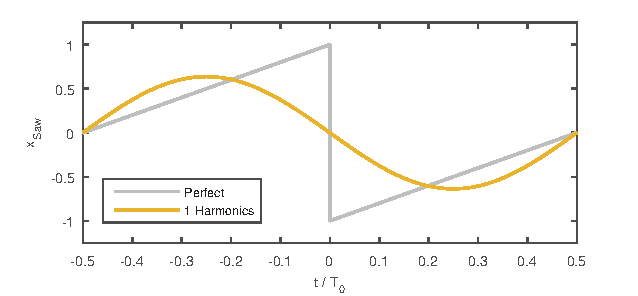
\includegraphics{AdditiveSynthesisSaw-1.pdf}
                    \end{figure}
                \addreference{{matlab source: \href{https://github.com/alexanderlerch/ACA-Slides/blob/master/matlab/displayAdditiveSynthesis.m}{matlab/displayAdditiveSynthesis.m}}}
            }
            
            \setcounter{i}{1}
            \whiledo{\value{i}<6}	
            {
                \pause
                \only<\value{beamerpauses}>
                {
                    \vspace{-4mm}
                    \begin{figure}
                        \centering
                        \includegraphics{AdditiveSynthesisSaw-\arabic{i}}
                    \end{figure}
                    \audioautoplay{additivesynthesis_saw_\arabic{i}}
                    
                    \addreference{{matlab source: \href{https://github.com/alexanderlerch/ACA-Slides/blob/master/matlab/displayAdditiveSynthesis.m}{matlab/displayAdditiveSynthesis.m}}}
                }
                \stepcounter{i} 
            }	
            
            \setcounter{i}{1}
            \whiledo{\value{i}<6}	
            {
                \pause
                \only<\value{beamerpauses}>
                {
                    \vspace{-4mm}
                    \begin{figure}
                        \centering
                        \includegraphics{AdditiveSynthesisRect-\arabic{i}.pdf}
                    \end{figure}
                    \audioautoplay{additivesynthesis_rect_\arabic{i}}
                    
                    \addreference{{matlab source: \href{https://github.com/alexanderlerch/ACA-Slides/blob/master/matlab/displayAdditiveSynthesis.m}{matlab/displayAdditiveSynthesis.m}}}
                }
                \stepcounter{i} 
            }	
        \end{frame}
        \begin{frame}{audio signals}{periodic signals 5/5}
            youtube example --- mechanical additive synthesis:
            
            \bigskip
            \bigskip
            \bigskip
            \bigskip
            \begin{center}
                \href{http://youtu.be/8KmVDxkia_w}{youtu.be/8KmVDxkia\_w}
            \end{center}
            %      
            \inserticon{video}
        \end{frame}

    \section[random signals]{random signals}
        \begin{frame}{audio signals}{random process 1/2}
            \textbf{random process}: ensemble of random series
            \figwithmatlab{RandomProcess}%{matlab/displayRandomProcess.m}
        \end{frame}

        \begin{frame}{audio signals}{random process 2/2}
            \begin{block}{random process}
                \begin{itemize}
                    \item   ensemble of random series
                    \item   each series represents a \textit{sample} of the process
                    \item   the following value is \textit{indetermined}, regardless of any amount of knowledge
                \end{itemize}
            \end{block}
            \begin{itemize}
                \item   special case: \textbf{stationarity}\\ statistical properties such as the mean are time invariant
                \item   example: white noise
            \end{itemize}
            \inserticon{lightbulb}
        \end{frame}

    \section[signal description]{description of (random) signals}
            \begin{frame}{statistical signal description}{probability density function}
                PDF $p_x(x)$
                \begin{itemize}
                    \item	abscissa: possible (amplitude) values
                    \item	ordinate: probability
                \end{itemize}
                \pause
                \begin{eqnarray*}
                    p_x(x)&\geq& 0 , and\\	
                    \int\limits_{-\infty}^{\infty}{p_x(x)\, dx} &=& 1	
                \end{eqnarray*}
                \pause
                RFD---Relative Frequency Distribution (sample of PDF)
                \begin{itemize}
                    \item[] histogram of (amplitude) values
                \end{itemize}
            \end{frame}	
            
            \begin{frame}{statistical signal description}{PDF examples}
                \question{What is the PDF of the following prototype signals:}
                \only<2>{
                \begin{itemize}
                    \item	square wave
                    \item	sawtooth wave
                    \item	sine wave
                    \item	white noise (uniform, gaussian)
                    \item	DC
                \end{itemize}}
                \only<3>{
                \figwithmatlab{PdfExamples}
                }
            \end{frame}
                
            \begin{frame}{statistical signal description}{RFD: real world signals}
                \figwithmatlab{Rfd}
            \end{frame}	

    \section{summary}
        \begin{frame}{summary}{lecture content}
            \begin{itemize}
                \item   signals can be categorized into \textbf{deterministic and random signals}
                    \begin{itemize}
                        \item   deterministic signal can be described in a mathematical function
                        \item   random processes can only be described by their general properties
                    \end{itemize}
                \bigskip
                \item      \textbf{periodic signals}
                    \begin{itemize}
                        \item   periodic signals are probably the most music-related deterministic signal
                        \item   any periodic (pitched) signal is a sum of weighted sinusoidals
                        \item   frequencies \textit{only} at the fundamental frequency and integer multiples
                    \end{itemize}
                \bigskip
                \item   \textbf{random} signals
                    \begin{itemize}
                        \item   noise, unpredictable
                    \end{itemize}
                \bigskip
                \item   \textbf{real-world} signals
                    \begin{itemize}
                        \item   can be seen as a time-varying mixture of these two signal categories
                    \end{itemize}
            \end{itemize}
            \inserticon{summary}
        \end{frame}
\end{document}
